\documentclass[12pt,a4paper,openright]{report}  %twoside
\let\openright=\cleardoublepage



%%% Choose a language %%%

\newif\ifEN
\ENtrue   % uncomment this for english
%\ENfalse   % uncomment this for czech

%%% Configuration of the title page %%%

\def\ThesisTitleStyle{mff} % MFF style
%\def\ThesisTitleStyle{cuni} % uncomment for old-style with cuni.cz logo
%\def\ThesisTitleStyle{natur} % uncomment for nature faculty logo

\def\UKFaculty{Faculty of Mathematics and Physics}

\def\UKName{Charles University in Prague} % this is not used in the "mff" style

% Thesis type names, as used in several places in the title
\def\ThesisTypeTitle{\ifEN BACHELOR THESIS \else BAKALÁŘSKÁ PRÁCE \fi}
\def\ThesisGenitive{\ifEN bachelor \else bakalářské \fi}
\def\ThesisAccusative{\ifEN bachelor \else bakalářskou \fi}

%%% Fill in your details %%%

\def\ThesisTitle{Virtual file system in user space}
\def\ThesisAuthor{{Milan Veselý}}
\def\YearSubmitted{2023}

% department assigned to the thesis
\def\Department{Katedra softwarového inženýrství}
% Is it a department (katedra), or an institute (ústav)?
\def\DeptType{Katedra}

\def\Supervisor{RNDr. Jakub Yaghob, Ph.D.}
\def\SupervisorsDepartment{Katedra softwarového inženýrství}

% Study programme and specialization
\def\StudyProgramme{Informatika}
\def\StudyBranch{Programování a vývoj software}

\def\Dedication{%
Dedication. \xxx{It is nice to say thanks to supervisors, friends, family, book authors and food providers.}
}

\def\AbstractEN{%
    This thesis presents a cross-platform Virtual File System (VFS) with versioning and encryption capabilities, implemented using the FUSE library in C++.
    The VFS adds password protection and encryption \ldots.
    Versioning allows users to access and restore previous file versions.
    The VFS is efficient and thoroughly tested, providing a reliable solution for secure file management \ldots
    This thesis demonstrates the successful implementation of a multiplatform VFS with unique features, allowing for secure and efficient file management across different devices.
}

\def\AbstractCS{%
    Tato práce se zabývá vývojem virtuálního souborového systému (VFS) s přidaným verzováním a šifrováním, implementovaný pomocí knihovny FUSE v jazyce C++.
    \ldots
}

% 3 to 5 keywords (recommended), each enclosed in curly braces.
% Keywords are useful for indexing and searching for the theses by topic.
\def\Keywords{%
        {VFS} {FUSE} {C++} {versioning} {security}
}

% If your abstracts are long and do not fit in the infopage, you can make the
% fonts a bit smaller by this setting. (Also, you should try to compress your abstract more.)
% Alternatively, consider increasing the size of the page by uncommenting the
% geometry modification in thesis.tex.
\def\InfoPageFont{}
%\def\InfoPageFont{\small}  %uncomment to decrease font size

\ifEN\relax\else
% If you are writing a czech thesis, you additionally need to fill in the
% english translation of the metadata here!
\def\ThesisTitleEN{\xxx{Thesis title in English}}
\def\DepartmentEN{\xxx{Name of the department in English}}
\def\DeptTypeEN{\xxx{Department}}
\def\SupervisorsDepartmentEN{\xxx{Superdepartment}}
\def\StudyProgrammeEN{\xxx{study programme}}
\def\StudyBranchEN{\xxx{study branch}}
\def\KeywordsEN{%
\xxx{{key} {words}}
}
\fi


\usepackage[a-2u]{pdfx}

\ifEN\else\usepackage[czech,shorthands=off]{babel}\fi
\usepackage[utf8]{inputenc}
\usepackage[T1]{fontenc}

% See https://en.wikipedia.org/wiki/Canons_of_page_construction before
% modifying the size of printable area. LaTeX defaults are great.
% If you feel it would help anything, you can enlarge the printable area a bit:
%\usepackage[textwidth=390pt,textheight=630pt]{geometry}
% The official recommendation expands the area quite a bit (looks pretty harsh):
%\usepackage[textwidth=145mm,textheight=247mm]{geometry}

%%% FONTS %%%
\usepackage{lmodern} % TeX "original" (this sets up the latin mono)

% Optionally choose an override for the main font for typesetting
\usepackage[mono=false]{libertinus} % popular for comp-sci (ACM uses this)
%\usepackage{tgschola} % Schoolbook-like (gives a bit of historic feel)
%\usepackage[scale=0.96]{tgpagella} % Palladio-like (popular in formal logic).

% Optionally choose a custom sans-serif fonts (e.g. for figures and tables).
% Default sans-serif font is usually Latin Modern Sans. Some font packages
% (e.g. libertinus) replace that with a better matching sans-serif font.
%\usepackage{tgheros} % recommended and very readable (Helvetica-like)
%\usepackage{FiraSans} % looks great
% DO NOT typeset the main text in sans-serif font!
% The serifs make the text easily readable on the paper.

% IMPORTANT FONT NOTE: Some fonts require additional PDF/A conversion using
% the pdfa.sh script. These currently include only 'tgpagella'; but various
% other fonts from the texlive distribution need that too (mainly the Droid
% font family).


% some useful packages
\usepackage{microtype}
\usepackage{amsmath,amsfonts,amsthm,bm}
\usepackage{graphicx}
\usepackage{xcolor}
\usepackage{booktabs}
\usepackage{caption}
\usepackage{floatrow}

% load bibliography tools
\usepackage[backend=bibtex,natbib,style=numeric,sorting=none]{biblatex}
% alternative with alphanumeric citations (more informative than numbers):
%\usepackage[backend=bibtex,natbib,style=alphabetic]{biblatex}
%
% alternatives that conform to iso690
% (iso690 is not formally required on MFF, but may help elsewhere):
%\usepackage[backend=bibtex,natbib,style=iso-numeric,sorting=none]{biblatex}
%\usepackage[backend=bibtex,natbib,style=iso-alphabetic]{biblatex}
%
% additional option choices:
%  - add `giveninits=true` to typeset "E. A. Poe" instead of full Edgar Allan
%  - `terseinits=true` additionaly shortens it to nature-like "Poe EA"
%  - add `maxnames=10` to limit (or loosen) the maximum number of authors in
%    bibliography entry before shortening to `et al.` (useful when referring to
%    book collections that may have hundreds of authors)
%  - for additional flexibility (e.g. multiple reference sections, etc.),
%    remove `backend=bibtex` and compile with `biber` instead of `bibtex` (see
%    Makefile)
%  - `sorting=none` causes the bibliography list to be ordered by the order of
%    citation as they appear in the text, which is usually the desired behavior
%    with numeric citations. Additionally you can use a style like
%    `numeric-comp` that compresses the long lists of citations such as
%    [1,2,3,4,5,6,7,8] to simpler [1--8]. This is especially useful if you plan
%    to add tremendous amounts of citations, as usual in life sciences and
%    bioinformatics.
%  - if you don't like the "In:" appearing in the bibliography, use the
%    extended style (`ext-numeric` or `ext-alphabetic`), and add option
%    `articlein=false`.
%
% possibly reverse the names of the authors with the default styles:
%\DeclareNameAlias{default}{family-given}

% load the file with bibliography entries
\addbibresource{refs.bib}

% remove this if you won't use fancy verbatim environments
\usepackage{fancyvrb}

% remove this if you won't typeset TikZ graphics
\usepackage{tikz}
\usepackage{tikz-uml}
\usetikzlibrary{positioning} %add libraries as needed (shapes, decorations, ...)

% remove this if you won't typeset any pseudocode
\usepackage{algpseudocode}
\usepackage{algorithm}

% remove this if you won't list any source code
\usepackage{listings}


\hypersetup{unicode}
\hypersetup{breaklinks=true}

\usepackage[noabbrev]{cleveref}
\usepackage{hyperref}


% various forms of TODOs (you should remove this before submitting)
\usepackage[textsize=tiny, backgroundcolor=yellow!25, linecolor=black!25]{todonotes}
\newcommand{\xxx}[1]{\textcolor{red!}{#1}}

 % remove this before compiling the final version


% use this for typesetting a chapter without a number, e.g. intro and outro
\def\chapwithtoc#1{
\chapter*{#1}
\addcontentsline{toc}{chapter}{#1}
}

% If there is a line/figure overflowing into page margin, this will make the
% problem evident by drawing a thick black line at the overflowing spot. You
% should not disable this.
\overfullrule=3mm

% The maximum stretching of a space. Increasing this makes the text a bit more
% sloppy, but may prevent the overflows by moving words to next line.
\emergencystretch=1em

\ifEN
\theoremstyle{plain}
\newtheorem{thm}{Theorem}
\newtheorem{lemma}[thm]{Lemma}
\newtheorem{claim}[thm]{Claim}
\newtheorem{defn}{Definition}
\theoremstyle{remark}
\newtheorem*{cor}{Corollary}
\else
\theoremstyle{plain}
\newtheorem{thm}{Věta}
\newtheorem{lemma}{Lemma}
\newtheorem{claim}{Tvrzení}
\newtheorem{defn}{Definice}
\theoremstyle{remark}
\newtheorem*{cor}{Důsledek}
\fi

\newenvironment{myproof}{
  \par\medskip\noindent
  \textit{\ifEN Proof \else Důkaz \fi}.
}{
\newline
\rightline{$\qedsymbol$}
}

% real/natural numbers
\newcommand{\R}{\mathbb{R}}
\newcommand{\N}{\mathbb{N}}

% asymptotic complexity
\newcommand{\asy}[1]{\mathcal{O}(#1)}

% listings and default lstlisting config (remove if unused)
\DeclareNewFloatType{listing}{}
\floatsetup[listing]{style=ruled}

\DeclareCaptionStyle{thesis}{style=base,font={small,sf},labelfont=bf,labelsep=quad}
\captionsetup{style=thesis}
\captionsetup[algorithm]{style=thesis,singlelinecheck=off}
\captionsetup[listing]{style=thesis,singlelinecheck=off}

% Uncomment for table captions on top. This is sometimes recommended by the
% style guide, and even required for some publication types.
%\floatsetup[table]{capposition=top}
%
% (Opinionated rant:) Captions on top are not "compatible" with the general
% guideline that the tables should be formatted to be quickly visually
% comprehensible and *beautiful* in general (like figures), and that the table
% "head" row (with column names) should alone communicate most of the content
% and interpretation of the table. If you just need to show a long boring list
% of numbers (because you have to), either put some effort into showing the
% data in an attractive figure-table, or move the data to an attachment and
% refer to it, so that the boredom does not impact the main text flow.
%
% You can make the top-captions look much less ugly by aligning the widths of
% the caption and the table, with setting `framefit=yes`, as shown below.  This
% additionally requires some extra markup in your {table} environments; see the
% comments in the example table in `ch2.tex` for details.
%\floatsetup[table]{capposition=top,framefit=yes}

\ifEN\floatname{listing}{Listing}
\else\floatname{listing}{Výpis kódu}\fi
\lstset{ % use this to define styling for any other language
  language=C++,
  tabsize=2,
  showstringspaces=false,
  basicstyle=\footnotesize\tt\color{black!75},
  identifierstyle=\bfseries\color{black},
  commentstyle=\color{green!50!black},
  stringstyle=\color{red!50!black},
  keywordstyle=\color{blue!75!black}}

% Czech versions of the used cleveref references (It's not as convenient as in
% English because of declension, cleveref is limited to sg/pl nominative. Use
% plain \ref to dodge that.)
\ifEN\relax\else
\crefname{chapter}{kapitola}{kapitoly}
\Crefname{chapter}{Kapitola}{Kapitoly}
\crefname{section}{sekce}{sekce}
\Crefname{section}{Sekce}{Sekce}
\crefname{subsection}{sekce}{sekce}
\Crefname{subsection}{Sekce}{Sekce}
\crefname{subsubsection}{sekce}{sekce}
\Crefname{subsubsection}{Sekce}{Sekce}
\crefname{figure}{obrázek}{obrázky}
\Crefname{figure}{Obrázek}{Obrázky}
\crefname{table}{tabulka}{tabulky}
\Crefname{table}{Tabulka}{Tabulky}
\crefname{listing}{výpis}{výpisy}
\Crefname{listing}{Výpis}{Výpisy}
\floatname{algorithm}{Algoritmus}
\crefname{algorithm}{algoritmus}{algoritmy}
\Crefname{algorithm}{Algoritmus}{Algoritmy}
\newcommand{\crefpairconjunction}{ a~}
\newcommand{\crefrangeconjunction}{ a~}
\fi
 % use this file for various custom definitions


\begin{document}

    % the layout is mandatory, edit only in dire circumstances

\pagestyle{empty}
\hypersetup{pageanchor=false}
\begin{center}

% top part of the layout, this actually differs between faculties

    \def\ThesisTitleXmff{%
        \ifEN
        \centerline{\mbox{
\includegraphics[width=166mm]{img/logo-en.pdf}}}
        \else
        \centerline{\mbox{
\includegraphics[width=166mm]{img/logo-cs.pdf}}}
        \fi
        \vspace{-8mm}\vfill%
        {\bf\Large\ThesisTypeTitle}
        \vfill%
        {\LARGE\ThesisAuthor}\par
        \vspace{15mm}%
        {\LARGE\bfseries\ThesisTitle}
        \vfill%
        \Department}
    \def\ThesisTitleCuniLogo#1{%
            {\large\UKName\par\medskip\par\UKFaculty }
        \vfill%
        {\bf\Large\ThesisTypeTitle}
        \vfill%
        \includegraphics[width=70mm]{#1}
        \vfill%
        {\LARGE\ThesisAuthor}\par
        \vspace{15mm}%
        {\LARGE\bfseries\ThesisTitle}
        \vfill%
        \Department\par}
    \def\ThesisTitleXcuni{\ThesisTitleCuniLogo{img/uklogo.pdf}}
    \def\ThesisTitleXnatur{\ThesisTitleCuniLogo{img/naturlogo.pdf}}

% choose the correct page and print it
    \csname ThesisTitleX\ThesisTitleStyle\endcsname
% latex corner: X is the new @

    \vfill

    {
        \centerline{\vbox{\halign{\hbox to 0.45\hsize{\hfil #}&\hskip 0.5em\parbox[t]{0.45\hsize}{\raggedright #}\cr
        \ifEN Supervisor of the \ThesisGenitive thesis:
        \else Vedoucí \ThesisGenitive práce: \fi
        & \Supervisor \cr
        \noalign{\vspace{2mm}}
        \ifEN Study programme: \else Studijní program: \fi
        & \StudyProgramme \cr
        \noalign{\vspace{2mm}}
        \ifEN Study branch: \else Studijní obor: \fi
        & \StudyBranch \cr
        }}}}

    \vfill

    \ifEN Prague \else Praha \fi
    \YearSubmitted

\end{center}

\newpage

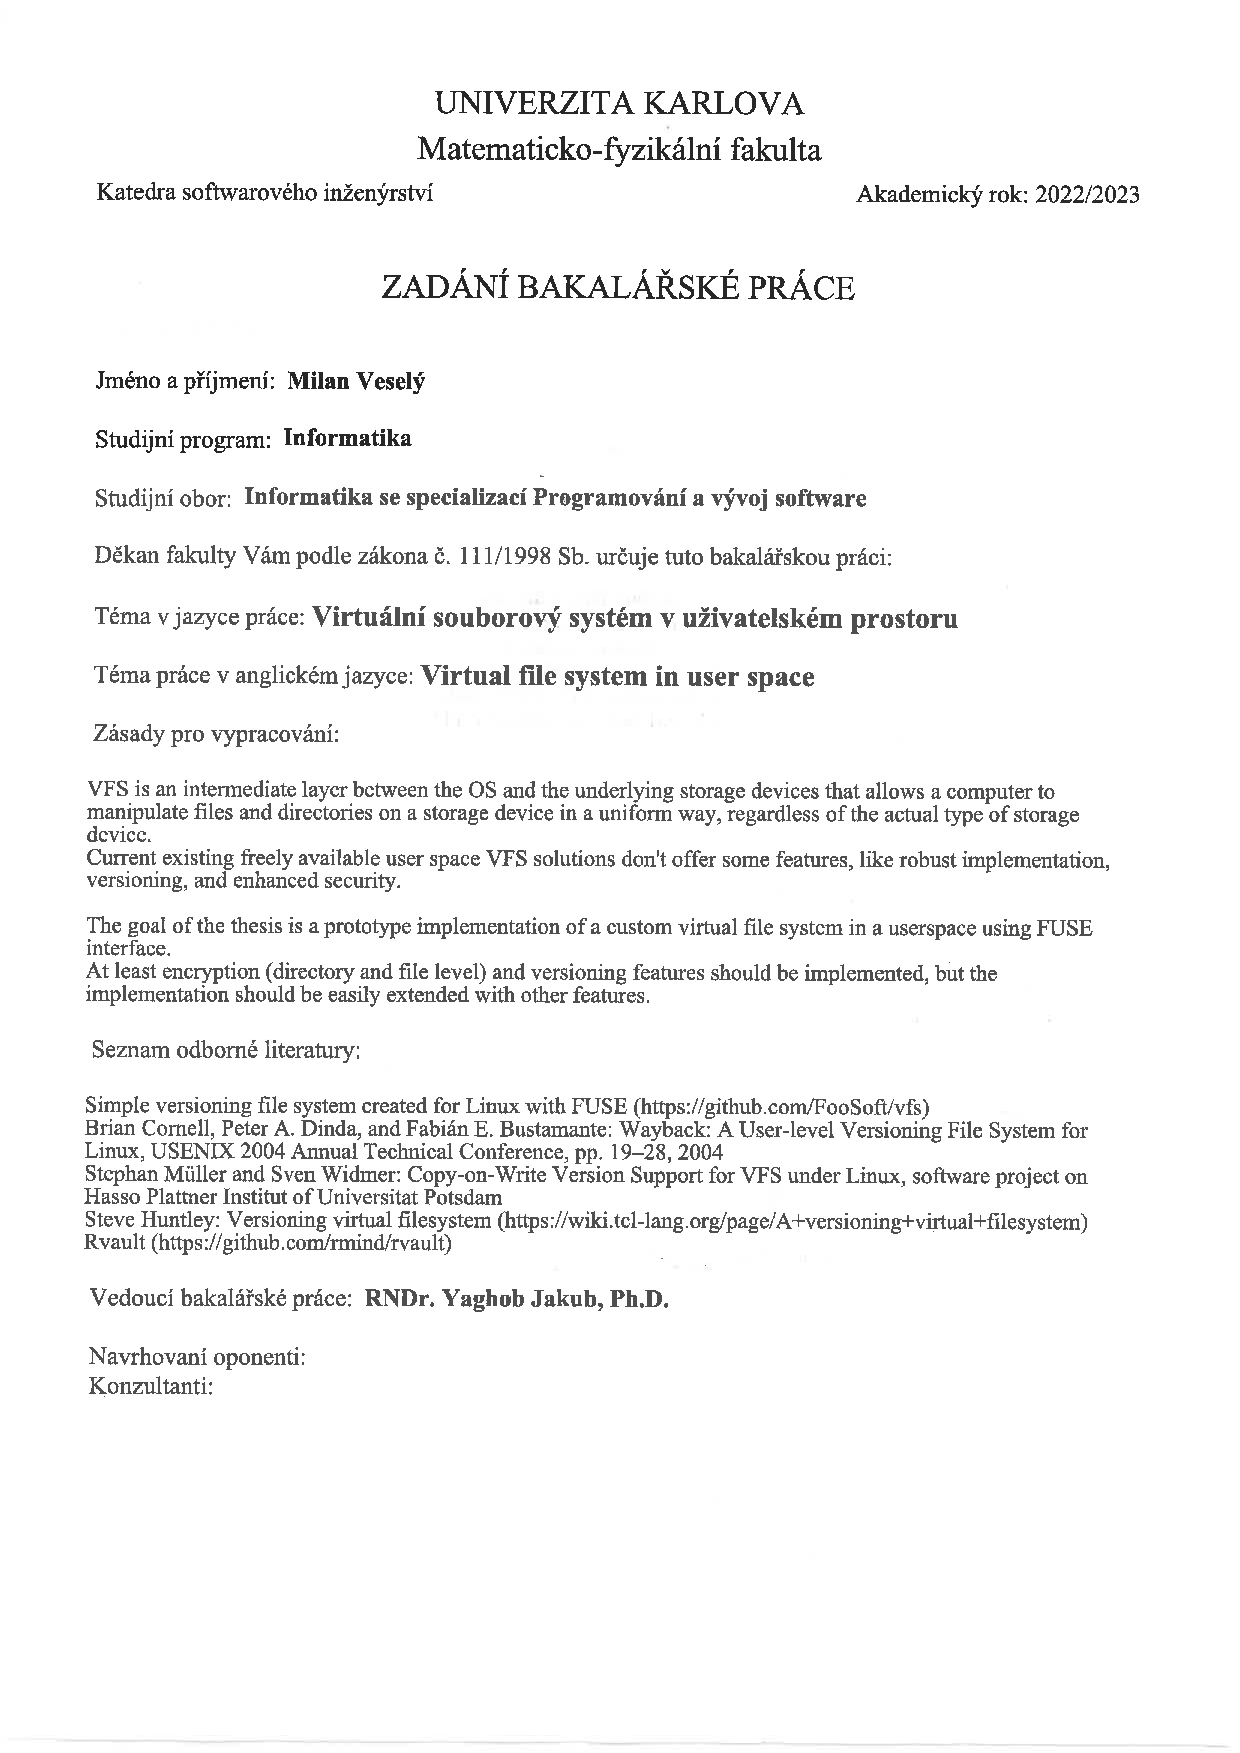
\includepdf[pages=-]{zadani.pdf}

% remember to sign this!
\openright
\hypersetup{pageanchor=true}
\pagestyle{plain}
\pagenumbering{roman}
\vglue 0pt plus 1fill

\ifEN
\noindent
I declare that I carried out this \ThesisAccusative thesis independently, and only with the cited
sources, literature and other professional sources. It has not been used to obtain another
or the same degree.
\else
\noindent
Prohlašuji, že jsem tuto \ThesisAccusative práci vypracoval(a) samostatně a výhradně
s~použitím citovaných pramenů, literatury a dalších odborných zdrojů.
Tato práce nebyla využita k získání jiného nebo stejného titulu.
\fi

\ifEN
\medskip\noindent
I understand that my work relates to the rights and obligations under the Act No.~121/2000 Sb.,
the Copyright Act, as amended, in particular the fact that the Charles
University has the right to conclude a license agreement on the use of this
work as a school work pursuant to Section 60 subsection 1 of the Copyright~Act.
\else
\medskip\noindent
Beru na~vědomí, že se na moji práci vztahují práva a povinnosti vyplývající
ze zákona č. 121/2000 Sb., autorského zákona v~platném znění, zejména skutečnost,
že Univerzita Karlova má právo na~uzavření licenční smlouvy o~užití této
práce jako školního díla podle §60 odst. 1 autorského zákona.
\fi

\vspace{10mm}


\ifEN
\hbox{\hbox to 0.5\hsize{%
    In \hbox to 6em{\dotfill} date \hbox to 6em{\dotfill}
    \hss}\hbox to 0.5\hsize{\dotfill\quad}}
\smallskip
\hbox{\hbox to 0.5\hsize{}\hbox to 0.5\hsize{\hfil Author's signature\hfil}}
\else
\hbox{\hbox to 0.5\hsize{%
    V \hbox to 6em{\dotfill} dne \hbox to 6em{\dotfill}
    \hss}\hbox to 0.5\hsize{\dotfill\quad}}
\smallskip
\hbox{\hbox to 0.5\hsize{}\hbox to 0.5\hsize{\hfil Podpis autora\hfil}}
\fi

\vspace{20mm}
\newpage

% dedication

\openright

\noindent
\Dedication

\newpage

% mandatory information page

\openright

\vbox to 0.49\vsize{\InfoPageFont
\setlength\parindent{0mm}
\setlength\parskip{5mm}

\ifEN Title: \else Název práce: \fi
\ThesisTitle

\ifEN Author: \else Autor: \fi
\ThesisAuthor

\DeptType:
\Department

\ifEN Supervisor: \else Vedoucí bakalářské práce: \fi
\Supervisor, \SupervisorsDepartment

\ifEN Abstract: \AbstractEN \else Abstrakt: \AbstractCS \fi

\ifEN Keywords: \else Klíčová slova: \fi
\Keywords

\vss}\ifEN\relax\else\nobreak\vbox to 0.49\vsize{\InfoPageFont
\setlength\parindent{0mm}
\setlength\parskip{5mm}

Title:
\ThesisTitleEN

Author:
\ThesisAuthor

\DeptTypeEN:
\DepartmentEN

Supervisor:
\Supervisor, \SupervisorsDepartmentEN

Abstract:
\AbstractEN

Keywords:
\KeywordsEN

\vss}
\fi

\newpage

\openright
\pagestyle{plain}
\pagenumbering{arabic}
\setcounter{page}{1}


    \tableofcontents

    
\chapwithtoc{Introduction}

As the significance of data continues to grow, multiple users require advanced features such as versioning or file-level encryption for their data storage.
This thesis presents a solution to this challenge by creating a virtual file system (VFS) that seamlessly integrates these features into existing file systems, enhancing their functionality with minimal effort from the user.
Specifically, the proposed VFS enables users to create snapshots for later rollbacks and effortlessly encrypt individual files or entire directories with a password, providing temporary decryption as needed.

Currently, users wanting the mentioned features must rely on separate programs.
For instance, versioning is often achieved through the well-known \texttt{git}, which creates a repository to store file changes in a \texttt{.git} directory, but this might be rather inconvenient in daily usage.
While there are a few file system-level versioning solutions available, they tend to be outdated, platform-specific, and difficult to use.
To password-protect files, users can choose from a wide array of software, such as Folder Lock, gpg or Encrypto, yet no single solution offers this particular feature at a lower level.

The primary issue with these programs, which this thesis seeks to address, lies in the necessity of accessing files through specialized software and exposing implementation details.
In contrast, the proposed VFS serves as an intermediate layer between the operating system and specific file systems, delivering the desired features in a more streamlined and user-friendly manner.

The subsequent chapters of this thesis will provide a in-depth examination of the virtual file system (VFS) concept, its functionality, and its internal mechanisms.
What analysis was performed to determine the feasibility of the project, and what design decisions were made to ensure the VFS's reliability and efficiency.
Additionally, following chapters will describe the methodology employed to incorporate versioning and file-level encryption, and techniques for utilizing the system's modularity to support additional features.
The thesis will end with an assessment of the VFS's performance, usability, and security to judge its overall effectiveness.
    \chapter{Theoretical overview}
\label{chap:refs}

The development of a custom Virtual File System (VFS) with modules for versioning and encryption capabilities requires an understanding of several key concepts and technologies.
This chapter aims to provide the necessary background and context to deeper understand the VFS implementation discussed in later chapters.
Even for those already familiar with the subject, a brief refresher might be helpful.


\section{Understanding File Systems}\label{sec:file-systems}

Let's start with what a file system is and what it does, as it is important for understanding the VFS itself.

A file system is a critical component of any operating system, tasked with managing and organizing data stored on a device.
As described by Oja et al.~\cite{oja-fs}, a filesystem represents the methods and data structures used by an operating system to maintain files on a disk or partition, that is, how files are organized on the disk.
This consists of multiple operations such as creation, reading, modifying, and deleting files or directories.
This is done in order to allow users and applications to interact seamlessly with the underlying storage medium.

It is important to distinguish between a disk or partition and the file system it contains.
While some programs operate directly on raw disk sectors or partitions, which could potentially damage or corrupt existing file systems, most programs interact with a file system.

There are various types of file systems, each tailored for specific operating systems and purposes.
Notable file systems include NTFS (New Technology File System) for Windows, HFS+ for macOS, and ext4 (fourth extended filesystem) for Linux.
Cross-platform compatibility can be attained using universal file systems like FAT32 or exFAT, which are compatible with multiple operating systems.

File systems employ diverse techniques to organize data, such as partitioning, allocation units, and indexing.
Additionally, file systems manage metadata, which is crucial for organizing and accessing stored data.
Metadata encompasses information such as file names, creation and modification timestamps, file sizes, and access permissions.


\section{Virtual File Systems}\label{sec:virtual-file-systems}

A Virtual File System (VFS) is an essential abstraction layer in modern operating systems, designed to ease the interaction between various file systems and user applications.
The VFS functions as an intermediary, enabling applications to access various file systems through a unified interface, regardless of the underlying file system's specific characteristics or structure.

According to a book by David A. Rusling~\cite{rusling-linux}, the VFS manages various mounted file systems by maintaining data structures that describe the entire virtual file system and the real mounted file systems.
The VFS uses superblocks and inodes, similar to the EXT2 file system, to describe files and directories within the system.
Each file system register with the VFS during operating system initialization.
File system modules are loaded as needed, allowing VFS to read their superblocks.
The VFS maintains a list of mounted file systems and their VFS superblocks, with each superblock containing pointers to specific file system functions.

The VFS inodes are traversed as the system's processes access directories and files.
Frequently accessed inodes are kept in the inode cache for quicker access.
Additionally, Linux VFS uses a common buffer cache, independent of the file systems, to cache data buffers from underlying devices.

VFS also plays a critical role in operating system design as it not only offers file system independence, but also provides benefits such as improved security or better performance.
In this thesis, I will also demonstrate that the extensibility of the VFS is a valuable advantage, enabling the incorporation of advanced features without requiring kernel modifications.

\subsection{VFS Operations}\label{subsec:vfs-operations}

The Virtual File System (VFS) provides a range of operations to interact with files and directories.
These operations are implemented as system calls, such as \texttt{open(2)}, \texttt{stat(2)}, \texttt{read(2)}, \texttt{write(2)}, and \texttt{chmod(2)}, which are called from a process context.

The way this is implemented in Linux VFS is described by an article by Richard Gooch and Pekka Enberg~\cite{vfs}.
During a system call, the VFS translates a pathname into a directory entry (dentry) by searching through the dentry cache.
However, if the cache is too small to fit all dentries in RAM, the VFS may have to create dentries and load inodes to resolve the pathname.
Each dentry typically has a pointer to an inode, which is a file system object that may be on disk or in memory.

When a file is opened, a file structure is allocated and initialized with a pointer to the dentry and file operation member functions taken from the inode data.
The \texttt{open()} file method is then called to enable the file system implementation to perform its work.
Finally, the file structure is placed into the file descriptor table for the process.

To read, write, and close files, the user-space file descriptor is used to call the appropriate file structure method.
As long as the file is open, the corresponding dentry and VFS inode remain in use.


\section{Encryption}\label{sec:encryption-approaches}

Another concept that has to be briefly discussed is encryption.
It is simply a process of applying cryptographic algorithms (encoding) to information in such a way that only authorized parties can access it.
In this thesis, I will use encryption as a means to transform the contents of files and directories into an unreadable format, which can only be deciphered with the appropriate decryption key.
Utilizing encryption enables users to effectively safeguard their data against unauthorized access, data breaches, and other malicious activities.

For file and directory encryption, symmetric key algorithms are commonly utilized due to their computational efficiency and robust security properties.
The Advanced Encryption Standard (AES) is a widely adopted option; however, in this thesis, the more modern and faster XChaCha20-Poly1305 algorithm has been chosen as the primary encryption method.
To derive an encryption key from a user-provided password, password-based key derivation functions will be implemented.

\subsection{XChaCha20-Poly1305}\label{subsec:xchacha20-poly1305}

XChaCha20-Poly1305 is an advanced symmetric encryption algorithm that combines the XChaCha20 stream cipher with the Poly1305 message authentication code (MAC).
This modern encryption algorithm is considered faster than AES, especially in software implementations, making it a suitable choice for this thesis~\cite{crypto_pp_xchacha20poly1305}.

The XChaCha20 stream cipher operates using a 256-bit secret key and a 192-bit nonce.
The increased nonce size in XChaCha20 significantly improves its resistance to nonce reuse attacks compared to the original ChaCha20 cipher.
The algorithm employs a series of simple operations, such as addition, rotation, and XOR, to generate a keystream, which is subsequently combined with the plaintext to produce the ciphertext.

To encrypt data using XChaCha20-Poly1305, a user first generates a secret key, which is a random sequence of 256 bits.
Then, the algorithm uses the secret key to transform the plaintext into ciphertext.
The ciphertext can only be decrypted back to its original plaintext form using the same secret key that was used to encrypt it.

\section{Versioning}\label{sec:versioning}

Versioning is simply a technique used to maintain multiple copies or states of a file or directory, allowing users to access and restore previous versions as needed.
It enables tracking of changes made to files over time, facilitating collaboration and recovery from accidental data loss or corruption.

Usually, versioning is implemented by storing multiple copies of a file or directory, each representing a different version.
This approach is straightforward and easy to implement, but it can be inefficient in terms of storage space and performance.
To address these issues, versioning can be implemented using a snapshot-based approach, which stores only the differences between versions, rather than storing multiple copies of the same file.
    \chapter{Analysis}
\label{chap:analysis}

\section{Alternatives}\label{sec:alternatives}

\xxx{From this point on, the document is a mess.}

Is it worth it?
What will it bring to the table\ldots

Non-virtual versioning file systems\ldots % have already been described on \href{https://en.wikipedia.org/wiki/Versioning_file_system}{Wikipedia}.

In addition, there are several virtual file systems (VFS) with versioning capabilities:

\begin{itemize}
\item There are two user space file systems written using FUSE:
\begin{itemize}
\item \href{https://github.com/FooSoft/vfs}{Simple versioning file system created for Linux with FUSE}, written in Go.
\item \href{https://www.usenix.org/legacy/events/usenix04/tech/freenix/cornell.html}{Wayback: A User-level Versioning File System for Linux}, which was written in Perl for the USENIX 2004 Annual Technical Conference using the old FUSE\@.
\end{itemize}
\item \href{https://osm.hpi.de/vvfs/}{Copy-on-Write Version Support for VFS under Linux} by Stephan Müller and Sven Widmer, implemented as a kernel patch.
\item \href{https://wiki.tcl-lang.org/page/A+versioning+virtual+filesystem}{A versioning virtual filesystem by Steve Huntley}, written with Tcl.
However, this is more of a language demonstration than a practical solution.
\end{itemize}

These products have various limitations, such as being Linux-only or being discontinued.
On the other hand, VFS with encryption is far less prevalent, although there are numerous non-virtual VFS with encryption capabilities, as documented on their \href{https://en.wikipedia.org/wiki/Encrypting_File_System}{Wikipedia page}.
The only example found that closely resembles the desired functionality is \href{https://github.com/rmind/rvault}{rvault}, which focuses on encrypting small files (passwords, keys, and secrets) and makes them available through one-time password authentication.
However, this differs from the intended functionality of this project.

Thus, the primary competition comes from higher-level applications that offer versioning and encryption functionality.
These applications come with their own set of drawbacks, such as the need to constantly run a background program (with access to all files) and limited extensibility for adding other features.
In most cases, incorporating additional features in these applications would not be feasible or practical.

\section{FUSE}\label{sec:fuse-analysis}

Even though There is an option to write kernel drivers\ldots

FUSE (Filesystem in Userspace) is a prominent library for creating a VFS in C++.
It enables developers to implement custom file systems in user space without modifying kernel code.
FUSE provides a comprehensive API for defining file system operations, making it a suitable choice for building a VFS in C++.
Although FUSE was initially designed for Linux, there are variants available for other platforms:

\begin{figure}[ht]
    \centering
    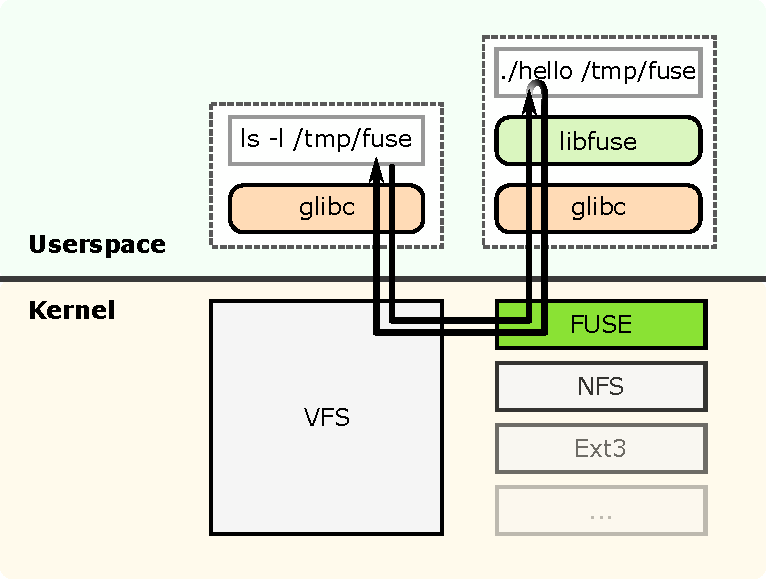
\includegraphics[width=\linewidth]{img/fuse_diagram}
    \caption{FUSE flow-chart diagram}
    \label{fig:fuse-diagram}
\end{figure}

\ldots

\begin{itemize}
\item \textbf{Linux}: \href{https://github.com/libfuse/libfuse}{libfuse} - The reference implementation of FUSE\@.
\item \textbf{macOS}: \href{https://osxfuse.github.io/}{FUSE for macOS} - A macOS port of FUSE\@.
\item \textbf{Windows}: \href{https://github.com/billziss-gh/winfsp}{WinFsp} - A Windows File System Proxy that provides FUSE-compatible functionality.
\end{itemize}

\section{Encryption}\label{sec:encryption-analysis}

\href{https://www.cryptopp.com/}{Crypto++} is a free C++ class library of cryptographic schemes.
It offers a wide range of cryptographic algorithms for encryption, hashing, and authentication.
Crypto++ can be used to implement file-level encryption within the VFS, ensuring data security and privacy.

\subsection{Gtest}\label{subsec:gtest}

\href{https://github.com/google/googletest}{Google Test} (also known as gtest) is a widely-used C++ testing framework developed by Google.

\ldots

\section{Basic idea of creating a VFS}\label{sec:basic-idea-of-creating-a-vfs}

\ldots

\section{Build system and multiplatform challenges}\label{sec:build-system-and-multiplatform-challenges}

Use of CMake, problem with M1 Mac and Windows\ldots even though portable
    \chapter{Design and Architecture}
\label{chap:design-and-architecture}


\section{Using FUSE in C++}\label{sec:fuse-in-cpp}

Incorporating FUSE in C++ presents many challenges, primarily due to its interface design, which necessitates the use of a static wrapper for operations.
The problem arises from FUSE expecting a C struct with pointers to functions, which poses a problem for non-static C++ methods.
To solve this issue, two solutions can be considered: either writing C++ code without utilizing objects, rendering the use of C++ instead of C rather pointless, or implementing a singleton wrapper with only static methods.

As is evident, the latter solution was chosen.
Fortunately, there was no need to start from scratch, as existing repositories already provide an incomplete solution to this problem.
The foundation for this project was built upon the fusexx~\cite{fusexx} repository, which was found most suitable for the needs of this thesis.

However, significant changes were made to the existing code, as it was not written in a modern C++ style and did not adhere to the project's design goals.
The first step was to refactor the code to use modern C++ features, such as removing C-style casts and similar.
Numerous warnings were resolved, and in some cases, methods were completely rewritten to improve readability and efficiency.

There was also a third, rather ``hacky'' solution, which involved beside other implementation details using a data field in the FUSE context to store a pointer to the C++ object.
Something similar is done in the fusepp~\cite{fusepp} repository.
But this approach didn't seem to be the most elegant solution, and it was decided to use the singleton wrapper instead.
Furthermore, the fusepp repository was not updated for several years and thus couldn't be used as a base for the project as opposed to fusexx.


\section{Architecture}\label{sec:architecture}

Once the foundation was laid, the next step was to design a core VFS\@.
It is important to note that this implementation was not the primary focus of this thesis as it was rather focused on providing modularity and extensibility.
The result of this is that the entire file system is built on top of already present filesystem in the operating system.
However, such implementation details can be easily replaced, allowing for future improvements.

Multiple approaches were contemplated: one involving a single VFS class and another comprising separate File, Directory, and VFS classes.
Although the latter approach adheres more closely to object-oriented principles, I have decided to go with the former, as it is better suited for use with FUSE as I will still need to somehow bound those classes into one.

\subsection{Modularity}\label{subsec:modularity}

The VFS is designed to be modular, allowing for the addition of new features without the need to modify the core implementation.
To achieve this, the decorator pattern is used.
The decorator pattern is a structural design pattern that involves a set of decorator classes used to wrap concrete components.
Decorator classes mirror the types of the components they decorate, sharing the same interface but adding or overriding behavior.

In the context of this project, the decorator pattern is utilized to add versioning and encryption features without modifying the core VFS implementation.
For example, an \texttt{EncryptionVfs} class is implemented as a decorator, inheriting from the \texttt{VfsDecorator} class.
The \texttt{VfsDecorator} class, in turn, inherits from the base \texttt{CustomVfs} class.
The decorator class wraps an instance of the base VFS class, allowing it to perform additional encryption-related tasks when reading or writing files.

Here is a simplified code of the decorator pattern used in this project:

\begin{lstlisting}[language=c++, basicstyle=\ttfamily\small]
class CustomVfs { /.../ };

class VfsDecorator : public CustomVfs {
public:
explicit VfsDecorator(CustomVfs& wrapped_vfs);

protected:
CustomVfs& wrapped_vfs_;
};

class EncryptionVfs : public VfsDecorator {
public:
explicit EncryptionVfs(CustomVfs& wrapped_vfs);

int read(/.../) override;
int write(/.../) override;

/.../

private:
CryptoPP::byte key_[CryptoPP::AES::DEFAULT_KEYLENGTH];
CryptoPP::byte iv_[CryptoPP::AES::BLOCKSIZE];
};
\end{lstlisting}

The \texttt{VfsDecorator} class wraps an instance of \texttt{CustomVfs} and can be extended by specific decorator implementations, such as \texttt{EncryptionVfs}.
This design allows for the seamless integration of new features, such as encryption or versioning, without modifying the core VFS implementation.

The use of this pattern is then demonstrated in the following code snippet, which shows how the VFS is initialized and used in the \texttt{main} function:

\begin{lstlisting}[language=c++, basicstyle=\ttfamily\small]
int main(int argc, char* argv[]) {
    CustomVfs custom_vfs();
    VersioningVfs versioned_vfs(custom_vfs);
    EncryptionVfs enc_vers_vfs(versioned_vfs);

    enc_vers_vfs.main(argc, argv);
    return 0;
}
\end{lstlisting}

Anyone can easily add new features to the VFS by implementing a new decorator class and wrapping it around the base VFS\@.

\subsection{Access to VFS features}\label{subsec:access-to-vfs-features}

A crucial aspect of the architecture is determining the method by which users can access the added VFS features.
In this implementation, hooks have been designed to integrate seamlessly with standard filesystem operations.
Additionally, a simple command-line interface (CLI) has been implemented to facilitate access to the VFS features, such as encryption and versioning.

These hooks function by intercepting attempts to read a file with a specific name.
The filesystem then captures this operation, performs the requested action, and returns the result as though it was read from the file.
This approach allows users to interact with the VFS features without deviating from standard filesystem operations.

The CLI consists of two primary components: one for encryption and another for versioning.
Users can execute commands related to these features via the CLI, making it a user-friendly and accessible interface for interacting with the VFS\@.
Commands for encryption may include encryption key management and selecting encryption algorithms, while versioning commands may involve creating new versions, listing available versions, and reverting to a previous version.

Although the current implementation utilizes a command-line interface, the hooks can potentially be integrated into a graphical user interface (GUI) in the future.
Incorporating the VFS features into a GUI would provide users with an even more intuitive and visually appealing interface for managing encryption and versioning.
However, the development of a GUI was beyond the scope of this thesis.

Benefits of this approach include the ability to easily integrate the VFS features into existing applications, such as file managers.
This is because the VFS features are accessed through standard filesystem operations, which are already supported by most applications.
Additionally, the hooks allow for the seamless integration of new features, such as encryption and versioning, without the need to modify the core VFS implementation as can be seen in the following code example:

\begin{lstlisting}[language=c++, basicstyle=\ttfamily\small]
int EncryptionVfs::read(const std::string &file_path,
                     char *buffer,
                     size_t size,
                     off_t offset) {
    if (is_encryption_hook(file_path)) {
        return handle_hook(file_path, buffer, size, offset);
    }

    // Do normal read operation...
}
\end{lstlisting}

Similarly, hooks can be implemented for the versioning feature, allowing users to interact with versioning functionality through standard filesystem operations.





    \chapter{Results and discussion}

Usability, performance impact, \ldots
    \chapter{Implementation}
\label{chap:implementation}

Once the preparation phase was complete, it was time to begin the implementation itself.


\section{Essential FUSE Operations}\label{sec:fuse-ops}

It was first essential to define and integrate various FUSE operations.
This section provides a brief overview of some of the essential operations, incorporating information from the Facile Engineering tutorial and IBM Developer article~\cite{ibm_fuse, facile_fuse}:

\begin{itemize}
    \item \textbf{getattr}: Retrieves the metadata of a given path.
    This operation is always called before any other operation made on the filesystem.
    It is responsible for reading the file or directory attributes, such as size, access permissions, and timestamps.
    \item \textbf{readdir}: Lists the contents of a directory, filling a buffer with the structure of the accessed directory.
    \item \textbf{mknod}: Creates a non-directory node, such as a file.
    \item \textbf{unlink}: Deletes a file.
    \item \textbf{open}: Called when the system requests a file to be opened.
    \item \textbf{read}: Called when FUSE is reading data from an opened file, while filling the buffer with the content of those bytes.
    \item \textbf{write}: Writes data to an open file.
    \item \textbf{mkdir}: Creates a new directory.
    \item \textbf{rmdir}: Deletes an existing directory.
    \item \textbf{rename}: Renames a file or directory.
\end{itemize}

Besides these operations a full-featured filesystem might need operations such as \texttt{truncate}, \texttt{symlink}, \texttt{link}, \texttt{chmod}, \texttt{chown}, \texttt{utime}, \texttt{statfs}, \texttt{flush}, \texttt{release}, \texttt{fsync}, \texttt{setxattr}, \texttt{getxattr}, \texttt{listxattr}, and \texttt{removexattr}.

To create a filesystem with FUSE, a structure variable of type fuse\_operations should be declared and passed to the fuse\_main function.
The fuse\_operations structure contains pointers to functions that will be called when the appropriate action is required.
This is, as described earlier\ref{sec:fuse-in-cpp}, done in the \texttt{FuseWrapper} class and all the other classes simply implement the required functions.

\subsection{Operations for the Base VFS}\label{subsec:base-ops}

The core of the implementation is provided by \texttt{CustomVfs} class, which is responsible for handling all file system operations.
This particular class mainly redirects the operations to the appropriate system calls, which are then handled by the operating system.
The exact way this is done is using a backing directory, which is mounted to the \texttt{.customvfs-{mount}} directory that is created when the filesystem is mounted.
This particular directory is then used to store all the files and directories that are created by the user by simply forwarding the operations to the backing directory.
Consequently, the debugging process is simplified as the user can easily access the backing directory and verify that the operations are being handled correctly.

Using the base VFS is also then as simple as creating an object and invoking the \texttt{main} method, as demonstrated in the following code snippet.\ref{lst:main}

\begin{lstlisting}[language=c++, basicstyle=\ttfamily\small, caption={Main method of the \texttt{CustomVfs} class.}, label={lst:main}]
int main(int argc, char* argv[]) {
    CustomVfs custom_vfs();
    custom_vfs.main(argc, argv);
    return 0;
}
\end{lstlisting}

The arguments passed to the \texttt{main} method are then simply forwarded to the wrapper and consequently to the FUSE library.
This allows the user to specify the mount point and other options such as the debug mode or ignoring non-empty mount point.


\section{Encryption}\label{sec:encryption}

To implement the prototype module of encryption, I have chosen to use the XChaCha20-Poly1305 as described in the initial chapter~\ref{subsec:xchacha20-poly1305}.
I particularly used this algorithm implemented by the libsodium library\ref{subsec:encryption-analysis}.

There are two main approaches to use the added encryption functionality.
The first approach is to use a user-defined password, which is then employed to generate the encryption key.
This method is not very practical, as the user has to manually lock and unlock files, since there is no mechanism to request the password when accessing a file.

The second approach involves using a key file.
This method is more convenient, as users can store the key file in a secure location and access their files without additional steps.
However, this brings up the question of when to encrypt and decrypt the files.

Encryption and decryption of files are easily performed upon opening and closing the file, respectively.
In contrast, handling directories is more complicated, as there is no way to identify when the directory is being accessed.
As a result, I have chosen to temporarily decrypt file names when reading the directory, while individual file contents are decrypted only when the file is opened.
This approach reduces unnecessary encryption and decryption operations and maintains relatively fast performance.

The encryption itself was done by asking the parent vfs for the proper file path and then using the libsodium library to encrypt or decrypt the file.
Encryption of directories was then done by simply encrypting the files and their names in the directory recursively.

\section{Versioning}\label{sec:versioning2}

The versioning module prototype is as of now rather limited since implementing a full-featured versioning system would be a significant undertaking.
Namely, instead of using a diff-based approach for versioning, I have chosen to store the entire file in the versioning system as it simplifies the implementation.
Diff-based approach could be then implemented in the future.

Similar to the encryption implementation, the read and write operations were wrapped to include versioning.
The following code snippet shows a high-level overview of how to wrap the write operation with versioning functionality.

\begin{lstlisting}[language=c++, basicstyle=\ttfamily\small]
int VersVfs::write(const std::string &file_path,
                   char *buf, size_t size, off_t off) {
    store_previous_version(file_path);
    if (off > 0) {
        prepare_newfile_for_write(file_path);
    }

    wrapped_vfs_->write(file_path, buf, size, off);
}
\end{lstlisting}

Meaning, the current version is always stored in a file with the real name, whereas the previous versions are suffixed with special symbol and their version number.
With this approach operations such as restore, delete, or list are relatively straightforward to implement.
Restore just creates a new stored version with the current content of the file and renames the restored version to the real name.
Delete operation then simply removes the file and all its versions.
And listing just finds all the files with the real name and the special symbol and returns them.
    \chapwithtoc{Conclusion and Future Work}

% The main goal of this thesis is thus to create a modular and easily extensible virtual file system (VFS) in user space as a comprehensive solution for these advanced storage needs.
% Created as a FUSE (Filesystem in Userspace) module using C++, the VFS should be able to be mounted irrespective of the underlying file system.
% The created VFS should also provide prototypes of modules for encryption and versioning, seamlessly integrating them into the core functionality with minimal user effort.
% Specifically, the proposed VFS prototypes should enable users to create snapshots for later rollbacks and let them easily encrypt individual files or entire directories with a password or key, providing temporary decryption as needed.
% Not to mention the fact that the VFS does not have the limitations of such program, as it can be mounted on top of any file system, including even a network file systems; and its features could also be easily layered on top of each other.
% However, this VFS is not intended to be a replacement for existing solutions, but rather a proof of concept that demonstrates the feasibility of creating a modular and extensible VFS\@.

This thesis demonstrated the reasonableness of implementing an extensible Virtual File System (VFS).
The developed VFS prototype is easily extensible and includes modules for versioning and encryption.
Although the current implementation may not be optimal, there is room for improvement.

\xxx{repeat goals}


Namely, there are several avenues for future development and research to further improve the results of this thesis:

\begin{itemize}
    \item \textbf{Optimization}: The current VFS implementation can be optimized for better performance, both in terms of storage efficiency and processing speed.
    \item \textbf{GUI Integration}: The VFS features can be integrated into a graphical user interface and even to some already existing file managers to provide users with an even more intuitive and visually appealing interface.
    \item \textbf{Additional Features}: New features or modules can be developed and integrated into the VFS, such as versioning based on diff, compression, deduplication, or support for different storage backends (e.g., cloud storage or distributed file systems).
    \item \textbf{Real-world Deployment}: The VFS can be further refined and tested for deployment in real-world scenarios, where its performance, reliability, and usability can be assessed in more diverse and demanding environments.
\end{itemize}

In conclusion, this thesis has demonstrated the viability of creating an extensible Virtual File System with support for encryption and versioning.
Future work can build upon this foundation to develop a more robust, performant, and feature-rich VFS suitable for a wide range of applications.
    
\ifEN
\chapwithtoc{Bibliography}
\else
\chapwithtoc{Seznam použité literatury}
\fi

\printbibliography[heading=none]


    \appendix
    %! suppress = MissingLabel
\chapter{Using this custom VFS}

\ldots

\section*{Compilation and setup}

On Debian-based Linux systems (such as Ubuntu), you may install these dependencies with APT:

\xxx{I will just copy-paste it from the final CI/CD script}

\begin{Verbatim}
apt-get install build-essential cmake libfuse-dev crypto++-dev ...
\end{Verbatim}

To unpack and compile the software, proceed as follows:

\begin{Verbatim}
...
cmake ..
\end{Verbatim}

\subsection*{Mount the file system}

Mounting the file system is rather simple.
All you need to do is a directory and to run the following command:

\begin{Verbatim}
  CustomVFS /path/to/mountpoint
\end{Verbatim}

\xxx{mby add notes about options}

\subsection*{Unmount the file system}

\begin{Verbatim}
  fusermount -u /path/to/mountpoint
\end{Verbatim}

\section*{Section}

Voila, you are all set.

Let's just learn how to use it\ldots

% if your attachments are complicated, describe them in a separate appendix
%\include{attachments}

    \openright
\end{document}
